\documentclass[
  11pt,
  letterpaper,
   addpoints,
   %answers
  ]{exam}

\usepackage{../exercise-preamble}
\usepackage{float}

\begin{document}

\noindent
\begin{minipage}{0.47\textwidth}

\includegraphics[width=\textwidth]{../fcfm_die}
\end{minipage}
\begin{minipage}{0.53\textwidth}
\begin{center} 
\large\textbf{Circuitos Eléctricos Analógicos} (EL3202-1) \\
\large\textbf{Clase auxiliar 2} \\
\normalsize Prof.~ Patricio Mendoza.\\
\normalsize Prof.~Aux.~Renato Planas ~Erik Sáez
\end{center}
\end{minipage}

\vspace{0.5cm}
\noindent
\vspace{.85cm}

\begin{questions}
    \question Preguntas teóricas.a
\begin{parts}
    \part Explique qué son las impurezas donadoras y las impurezas aceptoras.
    \part ¿A qué es igual el producto de $n_0$ y $p_0$?
    \part ¿De dónde provienen los huecos y electrones en un semiconductor para el caso intrínseco?
    \part Explique cómo se mueve la posición de la Energía de Fermi según se dope un semiconductor con átomos aceptores o átomos donadores.
    \part ¿Qué es la corriente de difusión? ¿Por qué esta corriente es $0$ si se dopa uniformemente un semiconductor?
\end{parts}

\begin{solution}
\subsection*{Resolución 1.1}
Las impurezas son átomos que se añaden intencionalmente a la red cristalina del semiconductor para modificar sus propiedades eléctricas. Los semiconductores puros como el silicio o germanio pertenecen al grupo IV de la tabla periódica y poseen 4 electrones de valencia.

\textbf{Impurezas donadoras:} Son átomos del grupo V de la tabla periódica (como fósforo, arsénico o antimonio) que poseen 5 electrones de valencia. Cuando estos átomos se incorporan a la red cristalina del semiconductor, 4 de sus electrones forman enlaces covalentes con los átomos vecinos de silicio, mientras que el quinto electrón queda débilmente ligado al átomo donador. A temperatura ambiente, este electrón adicional se libera fácilmente hacia la banda de conducción, creando un portador de carga negativo libre y dejando al átomo donador con carga positiva fija.

\textbf{Impurezas aceptoras:} Son átomos del grupo III de la tabla periódica (como boro, aluminio o galio) que poseen solo 3 electrones de valencia. Al incorporarse a la red cristalina, estos átomos forman solo 3 enlaces covalentes con los átomos vecinos, dejando un enlace incompleto. Este enlace incompleto puede aceptar fácilmente un electrón de un átomo vecino, creando un hueco (portador de carga positivo) en la banda de valencia y dejando al átomo aceptor con carga negativa fija.
\begin{figure}[H]
    \centering
    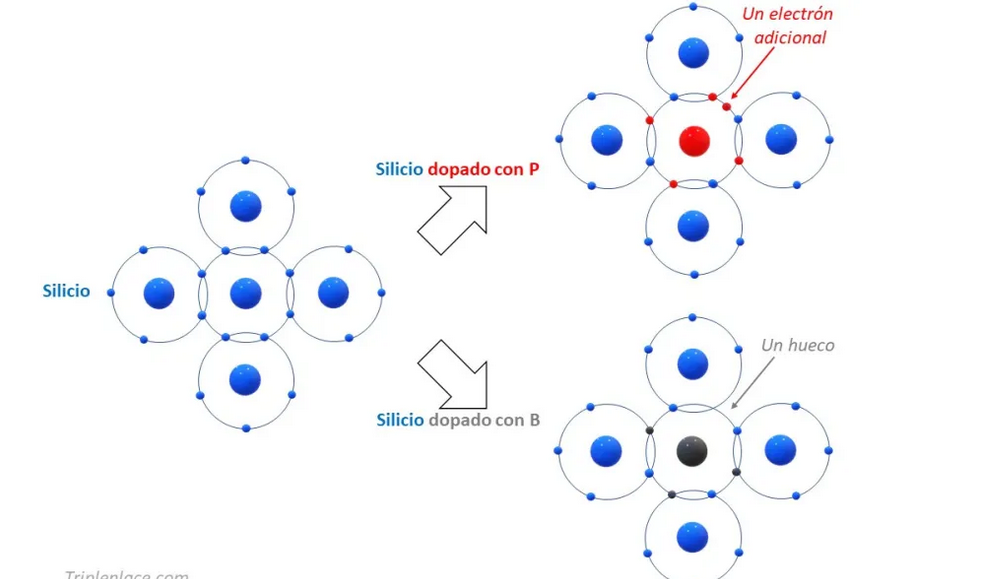
\includegraphics[width=0.8\textwidth]{../figures/Auxiliar_2_3}
    \caption{Representación atómica del silicio puro y dopado. Se muestra: (izquierda) silicio puro con enlaces covalentes completos, (arriba derecha) silicio dopado con fósforo (P) donde se observa un electrón adicional libre, y (abajo derecha) silicio dopado con boro (B) donde se forma un hueco por la falta de un electrón en el enlace covalente.}
    \label{fig:impurezas}
\end{figure}

Como se muestra en la Figura \ref{fig:impurezas}, cuando el silicio se dopa con fósforo (impureza donadora), el átomo de fósforo aporta un electrón adicional que queda libre para conducir. Por el contrario, cuando se dopa con boro (impureza aceptora), se crea un hueco en la estructura de enlaces covalentes debido a que el boro solo tiene 3 electrones de valencia.
\subsection*{Resolución 1.2}
El producto de las concentraciones de portadores de carga en un semiconductor está dado por la ley de acción de masas la cual se expresa como:
\begin{equation}
  n_0 p_0 = n_i^{2}  
\end{equation}
Donde se definen las siguientes variables:
\begin{itemize}
    \item $n_0$: Concentración de electrones libres en la banda de conducción en    equilibrio térmico [cm$^{-3}$]
    \item $p_0$: Concentración de huecos en la banda de valencia en equilibrio térmico [cm$^{-3}$]
    \item $n_i$: Concentración intrínseca de portadores de carga del semiconductor puro [cm$^{-3}$]
\end{itemize}

Esta relación es fundamental porque:
\begin{enumerate}
    \item Es válida tanto para semiconductores intrínsecos como dopados
    \item Se cumple bajo condiciones de equilibrio térmico
    \item Permite calcular una concentración conociendo la otra
\end{enumerate}

Se pueden realizar algunas aproximaciones útiles las cuales vienen dadas por:
\begin{itemize}
    \item Para \textbf{material tipo N} (dopado con impurezas donadoras):
    \begin{equation}
        n_0 \approx N_d \quad \text{y} \quad p_0 \approx \frac{n_i^2}{N_d}
    \end{equation}
    \item Para \textbf{material tipo P} (dopado con impurezas aceptoras):
    \begin{equation}
        p_0 \approx N_a \quad \text{y} \quad n_0 \approx \frac{n_i^2}{N_a}
    \end{equation}
\end{itemize}

Estas aproximaciones vienen del hecho que en un semiconductor fuertemente dopado, la concentración del portador mayoritario es aproximadamente igual a la concentración de impurezas dopantes (ignorando la concentración que existía previamente), mientras que la concentración del portador minoritario se determina por la ley de acción de masas.

\subsection*{Resolución 1.3}
En un semiconductor intrínseco (puro, sin impurezas), los huecos y electrones provienen exclusivamente de la \textbf{generación térmica de pares electrón-hueco}. A temperatura ambiente y superior, la energía térmica ($kT$, donde $k$ es la constante de Boltzmann y $T$ la temperatura absoluta) proporciona suficiente energía para que algunos electrones de valencia superen la banda prohibida (\emph{band gap}) y salten de la banda de valencia a la banda de conducción.

\begin{figure}[H]
    \centering
    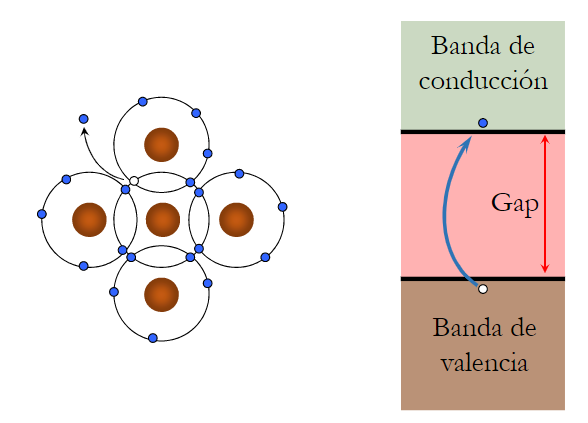
\includegraphics[width=0.7\textwidth]{../figures/Auxiliar_2_4}
    \caption{Generación térmica de pares electrón-hueco en un semiconductor intrínseco. (Izquierda) Representación atómica mostrando un electrón (azul) que absorbe energía térmica y se libera de un enlace covalente. (Derecha) Diagrama de bandas de energía ilustrando cómo un electrón supera el gap energético para pasar de la banda de valencia a la banda de conducción, dejando un hueco en la banda de valencia.}
    \label{fig:generacion_termica}
\end{figure}

Como se ilustra en la Figura \ref{fig:generacion_termica}, el proceso de generación térmica involucra:
\begin{enumerate}
    \item Un electrón de valencia absorbe energía térmica suficiente ($E \geq E_g$)
    \item El electrón salta de la banda de valencia a la banda de conducción
    \item Se crea simultáneamente un hueco en la banda de valencia
\end{enumerate}



\subsection*{Resolución 1.4}
La energía de Fermi ($E_F$) es un concepto fundamental en la física de semiconductores que representa el nivel energético que separa los estados ocupados de los vacíos a temperatura de cero absoluto (0 K). A 0 K, todos los estados de energía por debajo del nivel de Fermi están completamente ocupados por electrones, mientras que todos los estados por encima están completamente vacíos. A temperaturas finitas, esta distribución se suaviza según la distribución de Fermi-Dirac.

\begin{figure}[H]
    \centering
    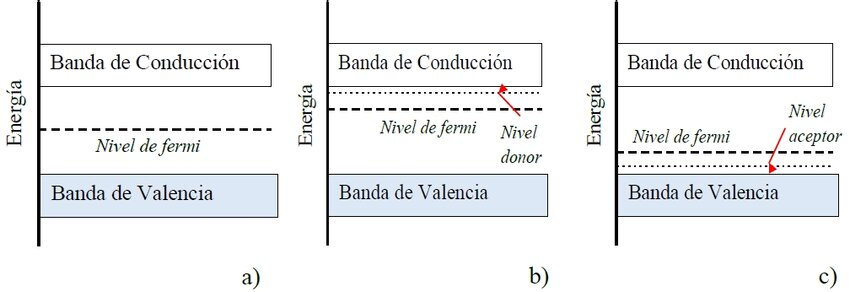
\includegraphics[width=0.8\textwidth]{../figures/Auxiliar_2_5}
    \caption{Diagrama de bandas de energía mostrando la posición del nivel de Fermi en diferentes tipos de semiconductores: a) semiconductor intrínseco, b) semiconductor tipo N (dopado con donadores), y c) semiconductor tipo P (dopado con aceptores).}
    \label{fig:fermi}
\end{figure}
Como se observa en la Figura \ref{fig:fermi}:

\textbf{a) Semiconductor intrínseco:}
\begin{itemize}
    \item El nivel de Fermi se ubica aproximadamente en el centro de la banda prohibida
    \item $E_F \approx E_i$ (nivel intrínseco)
    \item Las concentraciones de electrones y huecos son iguales: $n_0 = p_0 = n_i$
\end{itemize}

\textbf{b) Semiconductor tipo N (dopado con donadores):}
\begin{itemize}
    \item El nivel de Fermi se desplaza hacia la banda de conducción
    \item $E_F > E_i$ (por encima del nivel intrínseco)
    \item Mayor concentración de electrones: $n_0 > p_0$
    \item Los niveles donadores se ubican cerca de la banda de conducción
\end{itemize}

\textbf{c) Semiconductor tipo P (dopado con aceptores):}
\begin{itemize}
    \item El nivel de Fermi se desplaza hacia la banda de valencia
    \item $E_F < E_i$ (por debajo del nivel intrínseco)
    \item Mayor concentración de huecos: $p_0 > n_0$
    \item Los niveles aceptores se ubican cerca de la banda de valencia
\end{itemize}

\subsection*{Resolución 1.5}
La corriente de difusión es la corriente que se genera en un semiconductor debido al movimiento de portadores de carga (electrones y huecos) desde regiones de alta concentración hacia regiones de baja concentración. Este fenómeno ocurre cuando existe un gradiente de concentración en el material. Las Ecuaciones fundamentales de corriente de difusión corresponden a las siguientes:

\begin{itemize}
    \item Para electrones:
    \begin{equation}
        J_n = eD_n \frac{dn}{dx}
    \end{equation}
    \item Para huecos:
    \begin{equation}
        J_p = -eD_p \frac{dp}{dx}
    \end{equation}
\end{itemize}

Donde:
\begin{itemize}
    \item $J_n$: densidad de corriente de difusión de electrones [A/cm$^2$]
    \item $J_p$: densidad de corriente de difusión de huecos [A/cm$^2$]
    \item $e$: carga elemental del electrón ($1{,}6 \times 10^{-19}$ C)
    \item $D_n$: coeficiente de difusión de electrones [cm$^2$/s]
    \item $D_p$: coeficiente de difusión de huecos [cm$^2$/s]
    \item $\frac{dn}{dx}$: gradiente de concentración de electrones [cm$^{-4}$]
    \item $\frac{dp}{dx}$: gradiente de concentración de huecos [cm$^{-4}$]
\end{itemize}

Si se dopa uniformemente un semiconductor, la concentración de portadores es constante en todo el material. En este caso:
\begin{itemize}
    \item $\frac{dn}{dx} = 0$ (no hay gradiente de concentración de electrones)
    \item $\frac{dp}{dx} = 0$ (no hay gradiente de concentración de huecos)
\end{itemize}

Por tanto, según las ecuaciones anteriores, tanto $J_n = 0$ como $J_p = 0$, resultando en una corriente de difusión total nula. La corriente de difusión solo existe cuando hay variaciones espaciales en las concentraciones de portadores.
\end{solution}

%------
\question
Calcule las concentraciones de huecos y electrones en un material semiconductor de silicio que tiene una concentración intrínseca de $n_i = 10^{10}\,\text{cm}^{-3}$, cuando este material se encuentra a una temperatura de $293^\circ \text{K}$. Explicite en qué banda de energía se encuentra respectivamente cada tipo de partícula (hueco o electrón).
\begin{solution}
    \subsection*{Resolución 2.1}
Para un semiconductor intrínseco de silicio a temperatura $T = 293^\circ$K, debemos tener en cuenta que en un semiconductor intrínseco, cada electrón promovido a la banda de conducción deja exactamente un hueco en la banda de valencia. Por tanto, se debe cumplir la condición de neutralidad:

    \begin{equation}
        n_0 = p_0 = n_i = 10^{10}\,\text{cm}^{-3}
    \end{equation}

    donde las variables se definen como:
    \begin{itemize}
        \item $n_0$: concentración de electrones en equilibrio térmico
        \item $p_0$: concentración de huecos en equilibrio térmico  
        \item $n_i$: concentración intrínseca del material
    \end{itemize}

    La Figura \ref{fig:bandas_temp} ilustra este comportamiento: la excitación térmica permite que electrones (círculos azules) superen el gap energético y se ubiquen en la banda de conducción, mientras que los huecos resultantes (círculos rojos) permanecen en la banda de valencia.

    \begin{figure}[H]
        \centering
        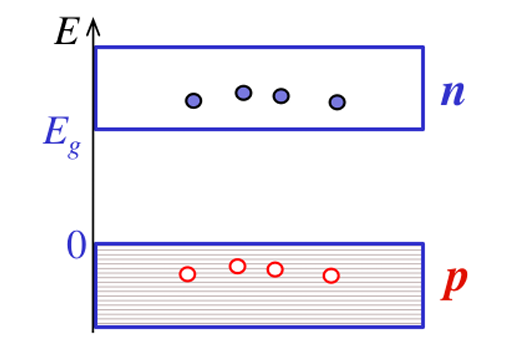
\includegraphics[width=0.6\textwidth]{../figures/Auxiliar_2_6}
        \caption{Bandas de energía en un semiconductor intrínseco con temperatura mayor que cero. Se observan electrones (círculos azules) en la banda de conducción y huecos (círculos rojos) en la banda de valencia debido a la excitación térmica.}
        \label{fig:bandas_temp}
    \end{figure}

\end{solution}
\question
Un material semiconductor está formado principalmente de silicio, con concentración intrínseca de $n_i = 10^{10}\,\text{cm}^{-3}$, pero dopado con partículas de fósforo con una concentración de $10^{17}\,\text{cm}^{-3}$. Cuando este material se encuentra a una temperatura de $293^\circ \text{K}$:
\begin{parts}
    \part Calcule las concentraciones de huecos y electrones utilizando el método exacto.
    \part Calcule las concentraciones de huecos y electrones utilizando el método aproximado.
    \part ¿Cuál es el error cometido al aproximar? ¿Qué ecuación no se cumple al hacer la aproximación?
    \part Explicite en qué banda de energía se encuentran respectivamente cada tipo de partícula (hueco o electrón).
    \part ¿Qué tipo de material es este semiconductor?
\end{parts}
\begin{solution}
    \subsection*{Resolución 3.1}
    En relación al enunciado tenemos los siguientes datos:
    \begin{itemize}
        \item Concentración intrínseca de silicio: $n_i=10^{10}\,\mathrm{cm^{-3}}$
        \item Concentración de donadores (fósforo): $N_D=10^{17}\,\mathrm{cm^{-3}}$
        \item Temperatura: $T=293\,$K
    \end{itemize}
    Utilizamos la ecuación de concentración de carga, la cual podemos entenderla como (Agregar interpretación intuitiva)
    \begin{equation}
        p + N_D = N_A + n
    \end{equation}
    Tenemos que conocemos la concentración de donadores $N_D$, pero dado que el material no fue dopado con aceptores, tendremos por tanto que $N_{A} = 0$. Por lo tanto se tendrá:
    \begin{equation}
        n = p + N_D.
    \end{equation}
    Dado que conocemos la concentración intrínseca $n_i=10^{10}\,\mathrm{cm^{-3}}$ podemos utilizar la ley de acción de masas:
    \begin{equation}
        n_i^2 = np = (10^{10})^2 = 10^{20}.
    \end{equation}
    Sustituyendo $n$ en la igualdad anterior obtenemos la ecuación cuadrática para $p$:
    \begin{align}
        n_i^2 &= p(p+N_D) \\
        10^{20} &= p^2 + N_D\,p \\
       0 &=  p^2 + 10^{17}p - 10^{20}.
    \end{align}
    Calculamos la raíz positiva dado que la concentración de huecos debe ser positiva.
    \begin{align}
        p &= \frac{-10^{17} \pm \sqrt{(10^{17})^2 + 4\cdot10^{20}}}{2} \\
          &= \frac{-10^{17} + 10^{10}\sqrt{10^{14}+4}}{2}\\
          &=10^{3}\,\mathrm{cm^{-3}}.
    \end{align}

    Finalmente,
    \begin{equation}
        n = p + N_D = 10^{3} + 10^{17} = 10^{17}\,\mathrm{cm^{-3}},
    \end{equation}
Con lo que se obtiene tanto la concentración de electrones como la de huecos:
\begin{align}
    n &=10^{17}\,\mathrm{cm^{-3}}, \\
    p &= 10^{3}\,\mathrm{cm^{-3}}.
\end{align}
\subsection*{Resolución 3.2}
    Aplicando el método aproximado $n \approx N_D$ (válido cuando $N_D\gg n_i$) y la ley de acción de masas se obtiene:
    \begin{equation}
        p = \frac{n_i^2}{n} \approx \frac{n_i^2}{N_D}
    \end{equation}

    Sustituyendo los valores numéricos:
    \begin{align}
        p &\approx \frac{(10^{10})^2}{10^{17}} = 10^{3}\,\mathrm{cm^{-3}}, \\
        n &\approx N_D = 10^{17}\,\mathrm{cm^{-3}}.
    \end{align}

    Estas aproximaciones coinciden con la solución exacta.
\subsection*{Resolución 3.3}

    La aproximación usada en la parte anterior, $n\approx N_D$, no cumple de forma estricta la ecuación de neutralidad de carga $p+N_D=N_A+n$ porque supone que la concentración de huecos es despreciable frente al dopaje. No obstante, para $N_D\gg n_i$ la contribución de $p$ es tan pequeña que la solución exacta de la cuadrática y la aproximación numérica coinciden dentro del margen de error del cálculo: $p\approx10^{3}\,\mathrm{cm^{-3}}$ y $n\approx10^{17}\,\mathrm{cm^{-3}}$. En consecuencia la aproximación es válida en este régimen y el error es insignificante para propósitos prácticos.
\subsection*{Resolución 3.4}
Se busca analizar la ubicación de los portadores de carga en las bandas de energía del semiconductor, por lo tanto tenemos que:
    \begin{itemize}
        \item \textbf{Electrones:} Se encuentran principalmente en la \textbf{banda de conducción} ($E > E_g$), donde actúan como portadores de carga móviles libres.
        \item \textbf{Huecos:} Se localizan en la \textbf{banda de valencia} ($E < 0$), representando estados vacíos que pueden participar en la conducción.
    \end{itemize}

    La Figura \ref{fig:tipo_n} muestra la estructura de bandas para un semiconductor tipo N con $T > 0$. Los electrones donados por las impurezas de fósforo ($N_D^+$) ocupan estados en la banda de conducción, mientras que los pocos huecos presentes se encuentran en la banda de valencia.

    \begin{figure}[H]
        \centering
        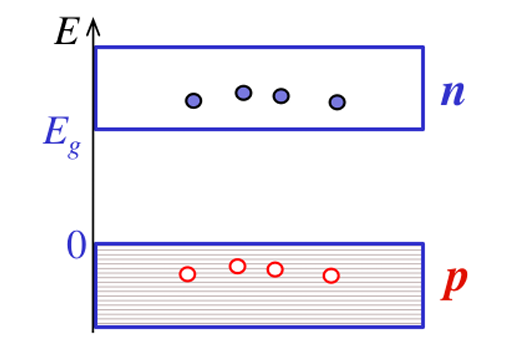
\includegraphics[width=0.5\textwidth]{../figures/Auxiliar_2_6}
        \caption{Diagrama de bandas de energía para semiconductor tipo N con $T > 0$. La banda de conducción contiene electrones (círculos azules) provenientes de los donadores ionizados $N_D^+$, mientras que la banda de valencia tiene pocos huecos (círculos rojos).}
        \label{fig:tipo_n}
    \end{figure}

\subsection*{Resolución 3.5}

    Dado que $n \gg p$ (con $n \approx 10^{17}\,\mathrm{cm^{-3}}$ y $p \approx 10^{3}\,\mathrm{cm^{-3}}$), este semiconductor es de \textbf{tipo N}, donde los electrones son los portadores mayoritarios y los huecos son los portadores minoritarios. La alta concentración de donadores ($N_D = 10^{17}\,\mathrm{cm^{-3}} \gg n_i = 10^{10}\,\mathrm{cm^{-3}}$) confirma que se trata de un material fuertemente dopado.
\end{solution}
\question
Un material semiconductor está formado principalmente de silicio pero que ha sido dopado en una parte con moléculas de Boro (parte gris de la Figura \ref{fig:p3}) con una concentración de $10^{16}\,\text{cm}^{-3}$ y dopado con partículas de fósforo con una concentración de $10^{17}\,\text{cm}^{-3}$ (parte blanca de la Figura \ref{fig:p3}). Recuerde que el silicio tiene una concentración intrínseca de $n_i = 10^{10}\,\text{cm}^{-3}$ cuando este material se encuentra operando a una temperatura de $293^\circ \text{K}$.

\begin{parts}
    \part ¿Qué tipo de materiales son cada parte dopada diferente?
    \part ¿Cuáles son las concentraciones de equilibrio en este material?
    \part ¿Existe un voltaje entre los dos tipos de materiales? Si es así, ¿cuál es el valor?
    \part ¿Qué representan las curvas verdes y azules en la Figura?, ¿qué representan la Abscisa y la Ordenada en la figura?
    \part Bosqueje un diagrama de bandas de energía para esta situación.
\end{parts}
\begin{solution}
    \subsection*{Resolución 4.1}
Se identifican los tipos de materiales dopados en la Figura \ref{fig:tabla_periodica}:
    \begin{figure}[H]
        \centering
        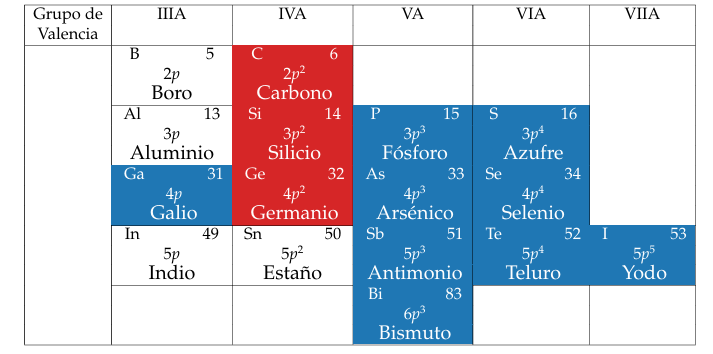
\includegraphics[width=0.8\textwidth]{../figures/Auxiliar_2_8.png}
        \caption{Extracto de la tabla periódica. Los átomos de Boro son del grupo IIIA, por lo tanto son átomos aceptores de electrones, mientras que los átomos de fósforo son del grupo VA y son átomos donadores de electrones.}
        \label{fig:tabla_periodica}
    \end{figure}
Según la tabla periódica (Figura \ref{fig:tabla_periodica}), identificamos los tipos de dopantes:
    \begin{itemize}
        \item \textbf{Boro (B):} Pertenece al grupo IIIA con 3 electrones de valencia ($2p^1$). Al sustituir un átomo de silicio (grupo IVA, 4 electrones de valencia), el boro crea un déficit de un electrón, formando un hueco. Por tanto, es una impureza aceptora.
        
        \item \textbf{Fósforo (P):} Pertenece al grupo VA con 5 electrones de valencia ($3p^3$). Al sustituir un átomo de silicio, el fósforo aporta un electrón adicional que queda libre. Por tanto, es una impureza donadora.
    \end{itemize}
Luego tendremos que los tipos de materiales resultantes:
    \begin{itemize}
        \item \textbf{Región dopada con Boro} (región izquierda): Semiconductor \textbf{tipo P}, donde los huecos son portadores mayoritarios con concentración $N_A = 10^{16}\,\mathrm{cm^{-3}}$.
        
        \item \textbf{Región dopada con Fósforo} (región derecha): Semiconductor \textbf{tipo N}, donde los electrones son portadores mayoritarios con concentración $N_D = 10^{17}\,\mathrm{cm^{-3}}$.
    \end{itemize}
    \subsection*{Resolución 4.2}
    
    Para calcular las concentraciones de equilibrio en cada región utilizamos la aproximación de que la concentración mayoritaria en el material es igual a la concentración de dopado. En el material n la concentración de electrones se aproxima a la concentración de dopado de partículas de fósforo, y en el material p la concentración de huecos se aproxima a la concentración de moléculas de Boro. Si reemplazamos los valores de las concentraciones de dopado en la ecuación de la ley de acción de masas (ecuación 1), podemos obtener las concentraciones restantes.

    \textbf{Para la región tipo N (dopada con fósforo):}
    \begin{align}
        n_n &\approx N_D = 10^{17}\,\text{cm}^{-3} \\
        p_n &= \frac{n_i^2}{n_n} = \frac{(10^{10})^2}{10^{17}} = \frac{10^{20}}{10^{17}} = 10^3\,\text{cm}^{-3}
    \end{align}

    \textbf{Para la región tipo P (dopada con boro):}
    \begin{align}
        p_p &\approx N_A = 10^{16}\,\text{cm}^{-3} \\
        n_p &= \frac{n_i^2}{p_p} = \frac{(10^{10})^2}{10^{16}} = \frac{10^{20}}{10^{16}} = 10^4\,\text{cm}^{-3}
    \end{align}

    \subsection*{Resolución 4.3}
    
    Se transportan huecos desde el material tipo p al material tipo n, y a su vez se transportan electrones desde el material tipo n al material tipo p. Esto genera una diferencia de potencial $V_o$ con su valor mayor en el material tipo n y su valor menor en el material tipo p. Este voltaje inhibe la difusión de electrones y huecos entre los materiales.

    \begin{align}
        V_o &= V_T \cdot \ln\left(\frac{n_n}{n_p}\right) = 25\,\text{mV} \cdot \ln\left(\frac{10^{17}\,\text{cm}^{-3}}{10^4\,\text{cm}^{-3}}\right) \approx 0{,}75\,\text{V}
    \end{align}

    \begin{align}
        V_o &= V_T \cdot \ln\left(\frac{p_p}{p_n}\right) = 25\,\text{mV} \cdot \ln\left(\frac{10^{16}\,\text{cm}^{-3}}{10^3\,\text{cm}^{-3}}\right) \approx 0{,}75\,\text{V}
    \end{align}
Donde tenemos que $V_{t} = \frac{kT}{q} = \frac{D_{e}}{\mu_{e}} = \frac{D_{h}}{\mu_{h}} \approx 25\,\text{mV}$. La cual se denomina la relacion de Einstein.
    \subsection*{Resolución 4.4}
    
    Las curvas verdes y azules en la figura representan las concentraciones de portadores de carga en función de la posición espacial en la unión p-n:

    \begin{itemize}
        \item \textbf{Curva verde}: Representa la concentración de electrones en función del espacio, $n(x)$
        \item \textbf{Curva azul}: Representa la concentración de huecos en función del espacio, $p(x)$
    \end{itemize}

    En cuanto a los ejes de la figura:
    \begin{itemize}
        \item \textbf{Abscisa (eje X)}: Posición espacial a lo largo de la unión p-n
        \item \textbf{Ordenada (eje Y)}: Concentraciones de portadores de carga ($n, p$)
    \end{itemize}

    Como se observa en la Figura \ref{fig:concentraciones_pn}, en la región tipo n (lado izquierdo) la concentración de electrones $n_n$ es alta y constante, mientras que la concentración de huecos $p_n$ es baja. En la región tipo p (lado derecho) ocurre lo contrario: la concentración de huecos $p_p$ es alta y la concentración de electrones $n_p$ es baja. En la zona de transición (región de depleción) ambas concentraciones varían gradualmente.

    \begin{figure}[H]
        \centering
        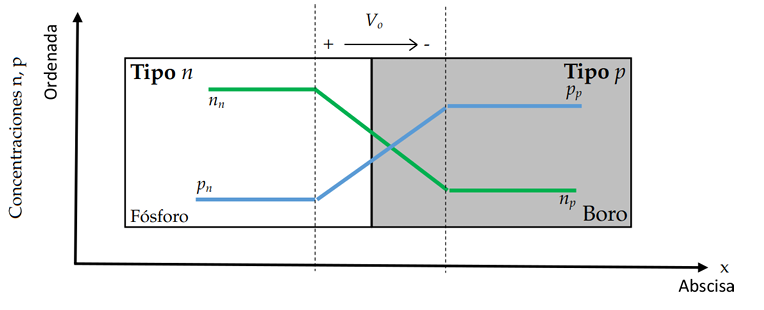
\includegraphics[width=0.8\textwidth]{../figures/Auxiliar_2_9}
        \caption{Perfiles de concentración de portadores en una unión p-n. La línea verde representa la concentración de electrones en función del espacio $n(x)$, mientras que la línea azul representa la concentración de huecos en función del espacio $p(x)$. Se observa la transición gradual en la región de depleción entre las regiones tipo n y tipo p.}
        \label{fig:concentraciones_pn}
    \end{figure}

    \subsection*{Resolución 4.5}
    
    El diagrama de bandas de energía para la unión p-n en equilibrio térmico muestra la estructura energética del sistema. En la Figura \ref{fig:bandas_pn} se observa:

    \begin{itemize}
        \item \textbf{Banda de conducción}: Ubicada en la parte superior del diagrama, donde se encuentran los electrones libres (representados por círculos azules). Esta banda se curva hacia arriba en la región de deplexión.
        
        \item \textbf{Banda de valencia}: Ubicada en la parte inferior del diagrama, donde se encuentran los huecos (representados por círculos rojos). Esta banda se curva hacia abajo en la región de deplexión.
        
        \item \textbf{Energía de Fermi ($E_F$)}: Representada por la línea punteada horizontal, permanece constante a través de toda la estructura en equilibrio térmico.
        
        \item \textbf{Curvatura de bandas}: En la región de depleción (zona central), las bandas se curvan debido al campo eléctrico interno generado por las cargas ionizadas. Esta curvatura crea una barrera de potencial de altura $eV_0 \approx 0{,}75$ eV.
    \end{itemize}

    La diferencia de altura entre las bandas en las regiones tipo n y tipo p corresponde al voltaje de contacto calculado anteriormente ($V_0 \approx 0{,}75$ V).

    \begin{figure}[H]
        \centering
        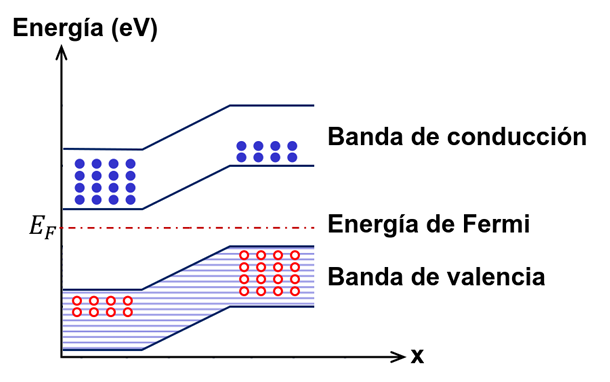
\includegraphics[width=0.8\textwidth]{../figures/Auxiliar_2_10}
        \caption{Diagrama de bandas de energía para una unión p-n en equilibrio térmico. Se muestran la banda de conducción, la banda de valencia, y la energía de Fermi ($E_F$). Los círculos azules representan electrones y los círculos rojos representan huecos. La curvatura de las bandas en la región de depleción crea una barrera de potencial.}
        \label{fig:bandas_pn}
    \end{figure}

\end{solution}
\begin{figure}[H]
    \centering
    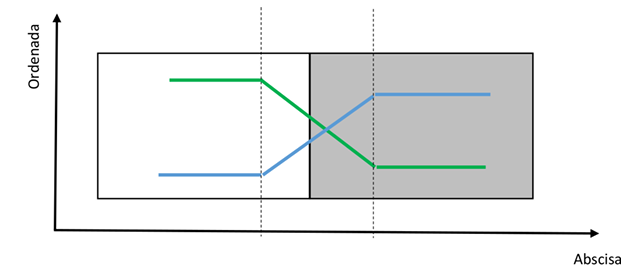
\includegraphics[width=0.7\textwidth]{../figures/Auxiliar_2_1}
    \caption{Problema 3}
    \label{fig:p3}
\end{figure}

\question
Para el mismo material del problema 3 ahora se ve que en la curva verde existe un cambio como se nota en la Figura \ref{fig:p4}:

\begin{parts}
    \part ¿Qué pudo haber producido este cambio?
    \part Si conociera el valor del punto rojo, ¿podría estimar el valor de la variable que está produciendo el cambio?
    \part ¿Qué necesitaría conocer para estimar la densidad de corriente asociada a esta curva? ¿Cuál sería su expresión si tuviera conocido todo lo que requiere?
    \part Bosqueje un diagrama de energía para esta situación.
\end{parts}

\begin{figure}[H]
    \centering
    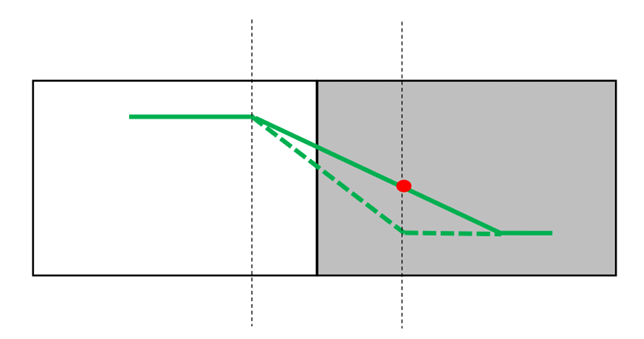
\includegraphics[width=0.7\textwidth]{../figures/Auxiliar_2_2}
    \caption{Problema 4}
    \label{fig:p4}
\end{figure}
\begin{solution}
    \subsection*{Resolución 5.1}

    El cambio observado en la curva verde se debe a la aplicación de un \textbf{voltaje externo} que está en contraposición al voltaje de contacto $V_o$. Con el voltaje mayor en el material tipo p y el menor en el material tipo n.

    \begin{figure}[H]
        \centering
        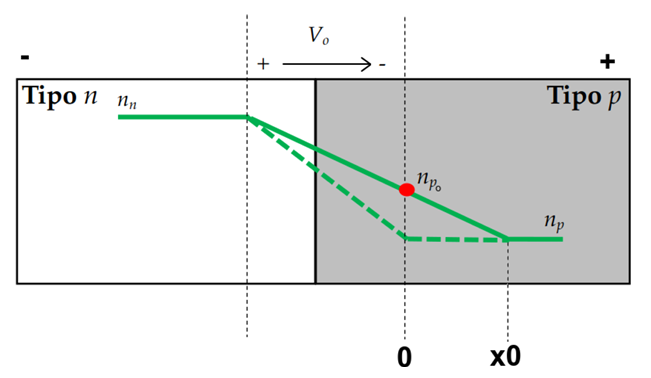
\includegraphics[width=0.8\textwidth]{../figures/Auxiliar_2_11}
        \caption{Voltaje externo aplicado con signo opuesto al voltaje de contacto $V_o$. Se observa cómo el perfil de concentración de electrones (línea verde sólida) se modifica comparado con el caso de equilibrio (línea verde punteada). El punto rojo indica la posición $x_0$ donde se produce el cambio más significativo.}
        \label{fig:voltaje_externo}
    \end{figure}

    Como se muestra en la Figura \ref{fig:voltaje_externo}, cuando se aplica un voltaje externo con polaridad opuesta al voltaje de contacto ($V_o$):

    \begin{itemize}
        \item El terminal positivo se conecta al lado tipo p
        \item El terminal negativo se conecta al lado tipo n
        \item Esta configuración reduce la barrera de potencial interna
        \item Se facilita el flujo de portadores mayoritarios a través de la unión
        \item La concentración de electrones en la región tipo p aumenta significativamente (línea verde sólida vs. punteada)
    \end{itemize}

    Esta condición corresponde a polarización directa del diodo p-n, donde el voltaje aplicado facilita la conducción de corriente al reducir la barrera energética que normalmente impide el flujo de portadores.

    \subsection*{Resolución 5.2}
    
    Conociendo el valor de $n_{p0}$ (concentración de electrones en la región p en el punto rojo), podemos estimar el voltaje externo $V$ que está causando el cambio en el perfil de concentración. Esta estimación se basa en las condiciones de borde bajo polarización (sesgo) aplicado.C uando se aplica un voltaje externo a la unión p-n, la concentración de electrones en la frontera de la región tipo p se relaciona con la concentración en equilibrio mediante:

    \begin{align*}
    n_n &= n_{p0}\,e^{\frac{V_0 - V}{V_T}} \\[4pt]
    \Rightarrow\quad
    n_{p0} &= n_n\,e^{\frac{V - V_0}{V_T}}
           = \underbrace{n_n\,e^{-\frac{V_0}{V_T}}}_{\displaystyle n_p\ }\,
             e^{\frac{V}{V_T}}
           = n_p\,e^{\frac{V}{V_T}} \\[6pt]
    \Rightarrow\quad
    V &= V_T \ln\!\left(\frac{n_{p0}}{n_p}\right).
    \end{align*}

    El factor $e^{\frac{V}{V_T}}$ indica el incremento exponencial en la concentración de portadores minoritarios debido al voltaje aplicado. Si $V > 0$ (polarización directa), la concentración $n_{p0}$ será mayor que la concentración de equilibrio $n_p$, lo que coincide con el comportamiento observado en la figura.



    \subsection*{Resolución 5.3}
    Recordemos que la corriente de difusión de electrones se debe al movimiento de electrones desde una región de alta concentración hacia una región de baja concentración. La expresión para la corriente de difusión de electrones es:   
    \begin{equation}
        J_{\text{DIFF-e}} = qD_n\frac{dn}{dx} \tag{3}
    \end{equation}

    Necesitamos calcular la variación de la concentración de electrones en el espacio ($dn/dx$). Para esto debemos modelar la caída de concentración entre el punto $x=0$ y el punto $x=x_0$, utilizando la ecuación de la recta:

    \begin{equation}
        (n - n_{p_0}) = -\frac{(n_{p_0} - n_p)(x - 0)}{x_0}
    \end{equation}

    \begin{equation}
        \Rightarrow n = -\frac{(n_{p_0} - n_p)}{x_0} \cdot x + n_{p_0}
    \end{equation}

    Luego, la derivada de la concentración de electrones en el espacio es:
    \begin{equation}
        \frac{dn}{dx} = -\frac{(n_{p_0} - n_p)}{x_0}
    \end{equation}

    Reemplazando en la ecuación (3) y utilizando lo calculado en la parte b:
    \begin{equation}
        J_{\text{DIFF-e}} = qD_n\left[-\frac{n_{p_0}e^{\frac{V}{V_T}} + n_p}{x_0}\right]
    \end{equation}

    \begin{equation}
        J_{\text{DIFF-e}} = -\frac{qD_nn_p}{x_0}\left(e^{\frac{V}{V_T}} - 1\right)
    \end{equation}

    Pero en el problema anterior vimos que $n_p = n_i^2/N_A$, entonces:
    \begin{equation}
        J_{\text{DIFF-e}} = -\frac{qD_nn_i^2}{x_0N_A}\left(e^{\frac{V}{V_T}} - 1\right)
    \end{equation}
    Donde recordemos que las variables involucradas corresponden a las siguientes:
    \begin{itemize}
        \item $q$: carga del electrón
        \item $D_n$: coeficiente de difusión de electrones
        \item $n_i$: concentración intrínseca
        \item $N_A$: concentración de aceptores
        \item $x_0$: ancho de la región de transición
        \item $V$: voltaje aplicado
        \item $V_T$: voltaje térmico
    \end{itemize}

    \subsection*{Resolución 5.4}
    
    El diagrama de bandas de energía para la unión p-n bajo polarización directa muestra los cambios en la estructura energética cuando se aplica un voltaje externo. Como se observa en la Figura \ref{fig:bandas_polarizacion}:

    \begin{figure}[H]
        \centering
        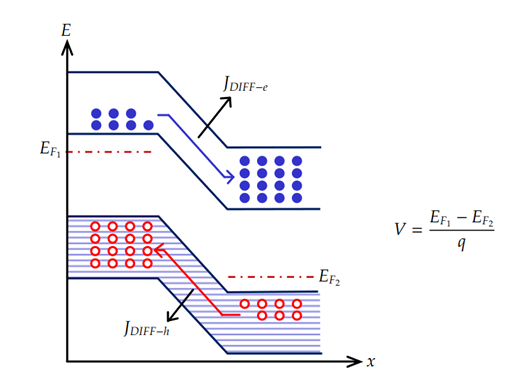
\includegraphics[width=0.6\textwidth]{../figures/Auxiliar_2_12}
        \caption{Diagrama de bandas de energía para una unión p-n bajo polarización directa. El voltaje externo cambia la estructura de la red cristalina, torciendo las bandas de energía. Los electrones del material tipo n ahora pueden moverse por difusión hacia el material tipo p, y a su vez, los huecos del material tipo p pueden moverse hacia el material tipo n. Esto se traduce en corrientes de difusión de electrones ($J_{\text{DIFF-e}}$) y de huecos ($J_{\text{DIFF-h}}$). Las diferencias entre las energías de Fermi dividida por la carga son equivalentes al voltaje externo.}
        \label{fig:bandas_polarizacion}
    \end{figure}

Algunas características del diagrama de bandas bajo polarización directa corresponden a lo siguiente:
    \begin{itemize}
        \item \textbf{Reducción de la barrera de potencial}: El voltaje aplicado reduce la altura de la barrera energética, facilitando el transporte de portadores.
        \item \textbf{Separación de niveles de Fermi}: Los niveles de Fermi en las regiones n y p se separan por una cantidad igual al voltaje aplicado: $V = \frac{E_{F1} - E_{F2}}{q}$.
        \item \textbf{Flujo de electrones}: Los electrones de la banda de conducción en la región n pueden difundirse hacia la región p, generando la corriente $J_{\text{DIFF-e}}$.
        \item \textbf{Flujo de huecos}: Los huecos de la banda de valencia en la región p pueden difundirse hacia la región n, generando la corriente $J_{\text{DIFF-h}}$.
        \item \textbf{Curvatura de bandas modificada}: La aplicación del voltaje externo modifica la curvatura natural de las bandas en la región de depleción
        \item \textbf{Inyección de portadores minoritarios}: Se inyectan electrones en la región p y huecos en la región n, aumentando las concentraciones de portadores minoritarios.
    \end{itemize}
    La condición $V = \frac{E_{F1} - E_{F2}}{q}$ establece la relación directa entre el voltaje aplicado externamente y la separación energética entre los niveles de Fermi de ambas regiones, confirmando que el sistema ya no está en equilibrio térmico.

\end{solution}
\end{questions}

\end{document}